\section{Ideas for games}
\begin{epigraph}
    \#долой\_hashtag'и
\end{epigraph}

\begin{itemize}
\item Идея для игры, где все противники главного героя умирают на его глазах из-за различных несчастных случаев или по собственному идиотизму.
Главный герой --- суицидник, который боится себя убивать и просит всех остальных, а они вместо этого гибнут сами, при попытках его убить.
\item Игра, где из-за маленькой оплошности совершенной в начале игры, в финале не может закончить игру (либо всё плохо заканчивается).
Как пример: забыл зарядить телефон, а в конце должен был получить инструкции по обезвреживанию бомбы через него.
\item iDivan.\\
Игра квест/рпг с элементами симс- главный герой должен выполнять разные миссии, но главное условие: он подзаряжается энергией лёжа на диване.
Уровень энергии падает пропорционально времени, проведённому не на диване. А ещё можно тюнинговать диван - но на ускорение зарядки это влиять
не будет (только понты).

\begin{figure}[ht!]
    \center
    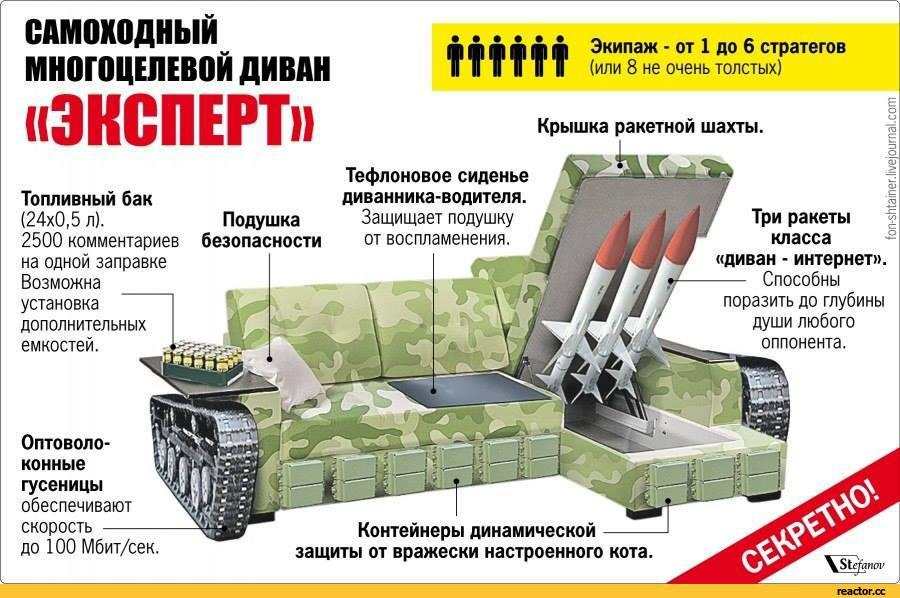
\includegraphics[width=.7\textwidth]{iDivan.jpg}
\end{figure}

\item Мини-игра: строитель адских котлов, для людей:
* ставящие неправильно ударение в словах\\
* неправильно ставящих машину\\
* неправильно согласующих падежи существительного и причастия "... для людей: ставящие неправильно ..."\\
* расставляющих лишние запятые\\
*запиливающих в беседы стикеры
\item on-real игра для тренировки дикции (основана на реальных событиях): пока вы громко отчётливо и грамматически правильно не произнесёте
требуемую фразу маршрутка не останавливается + можно также использовать не только тренировку дикции: решение задач, написание сочинений
и многое другое...
\end{itemize}
\begin{figure}[ht!]
    \centering
    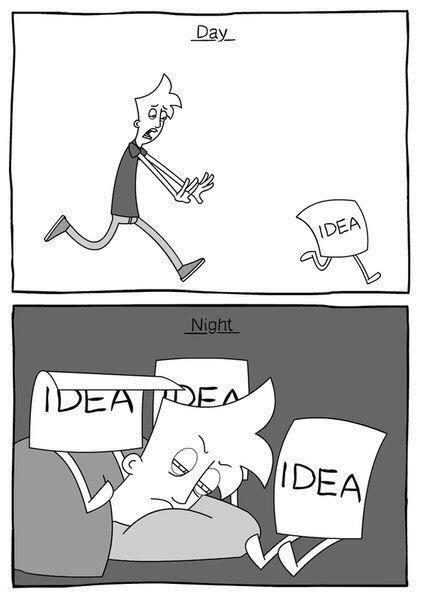
\includegraphics[height=13cm,width=8cm]{night}
    \caption{Люблю ночь}
\end{figure}
